\documentclass{article}

\title{Wspomaganie decyzji - Zad. 1}
\author{Artur Dziedziczak}
\date{\today}

\usepackage{microtype}
\usepackage[
    backend=biber,
    natbib=true,
    url=true,
    doi=true,
    eprint=false
]{biblatex}
\usepackage[a4paper, total={6in, 8in}]{geometry}

\addbibresource{sample.bib}
\usepackage{gensymb}
\usepackage{graphicx}

\usepackage{hyperref}
\hypersetup{
    colorlinks=true,
    linkcolor=blue,
    filecolor=magenta,
    urlcolor=cyan,
    pdftitle={Overleaf Example},
    pdfpagemode=FullScreen,
    }

\usepackage{float}

\usepackage[utf8]{inputenc}
\usepackage{amsthm}
\usepackage[english, polish]{babel}
\usepackage[T1]{fontenc}
\usepackage{theorem}
\usepackage{listings}

\lstset{frame=tb,
  language=Bash,
  aboveskip=3mm,
  belowskip=3mm,
  showstringspaces=false,
  columns=flexible,
  basicstyle={\small\ttfamily},
  numbers=none,
  numberstyle=\tiny\color{gray},
  keywordstyle=\color{blue},
  commentstyle=\color{dkgreen},
  stringstyle=\color{mauve},
  breaklines=true,
  breakatwhitespace=true,
  tabsize=3
}

\usepackage[justification=centering]{caption}
\begin{document}

\maketitle

\section{Zadanie projektu}

Rozważamy następujące uproszczone zagadnienie optymalizacji produkcji w systemie zamkniętym:
\begin{itemize}
    \item Należy osiągnąć możliwie największy zysk ze sprzedaży produktów: stali, maszyn, ciągników.
          Jednostkowa cena sprzedaży wynosi: 900 zł dla stali, 2500 zł dla maszyn, 4000 zł dla pierwszych 50 tys. ciągników, 3500 zł dla dalszych 25 tys.,
          3000 zł dla dalszych 75 tys. i 2700 zł dla dalszych ciągników.
    \item Na wyprodukowanie jednostki stali potrzeba: 0.05 jednostek maszyn, 0.08 jednostek ciągników, 0.5 jednostki pracy.
          Koszt produkcji wynosi 300 zł. Maksymalne możliwości produkcyne: 400 tys. jednostek.
    \item  Na wyprodukowanie jednoski maszyn potrzeba: 0.75 jednostek stali, 0.12 jednostek ciągników, 5 jednostki pracy. Koszt produkcji wynosi 150 zł. Maksymalne możliwości produkcyjne: 50 tys jednostek.
    \item Na wyprodukowanie jednostki ciągników potrzeba: 1 jednostkę stali, 0.1 jednostek maszyn, 3 jednostki pracy. Koszt produkcji wynosi 500 zł. Maksymalne możliwości produkcyne: 550 tys. jednostek.
    \item Dostępne zasoby pracy wynoszą 600 tys. jednostek.
\end{itemize}
\begin{enumerate}
    \item Sformulować możliwie najprostszy model programowania matematycznego dopuszczając podzielność jednostek produktów.
    \item Wyznaczyć rozwiązanie optymalne (przy pomocy dowolnie wybranego solwera) i zbadać jego wrażliwość na zmiany wielkości zasobu pracy.
    \item Jaki wpływ na rozwiązanie optymalne miałoby dodatkowe wymaganie pelnego wykorzystania zasobów pracy?
    \item Jakie są ograniczenia i jakie możliwości rozszerzania opracowanego modelu?
\end{enumerate}

\noindent
Raport z wykonania zadania powinien zawierać:

\begin{enumerate}
    \item Analityczne sformułowanie modelu. Specyfikacje problemu decyzyjnego z do-określeniem wszystkich elementów. Określenie zmiennych decyzyjnych, ograniczeń i funkcji celu.
    \item Rozwiązanie zadania i interpretacja uzyskanych wyników. Sformułowanie modelu/zadania w postaci do rozwiązania wybranym solwerem.  Wyznaczenie , rozwiązania i interpretacja wyników w terminach oryginalnego modelu.
    \item Analiza wrażliwości rozwiązania za zmiany danych. Należy przeprowadzić analizę,skutków zmian wielkości zasobu pracy.
    \item Analiza możliwości rozszerzania modelu. Opis projektu koncentruje się , na opisie uproszczonej sytuacji decyzyjnej. Przedyskutować możliwości rozszerzenia modelu urealniające jego zastosowanie wskutek uwzględnienia większej liczby zależności itp.
      Przeanalizować ewentualne skutki takich rozszerzeń dla zadania obliczeniowego.
\end{enumerate}

Ocenie podlegają , wszystkie wymienione punkty oraz jakość raportu.
Raport powinien być plikiem pdf (z ewentualnymi załącznikami).

\section{Analityczne sformułowanie modelu. Specyfikacje problemu decyzyjnego z do określeniem wszystkich elementów. Określenie zmiennych decyzyjnych, ograniczeń i funkcji celu.}

\noindent
Formułowanie problemu zaczynam od stworzenia modelu matematycznego.

\noindent
Po przeczytaniu problemu nasunęły mi się następujące spostrzeżenia:

\begin{itemize}
	\item Ograniczenia, które w przedstawionym zagadnieniu są liniowe.
	\item Ceny ciągników można zamodelować przedziałami metodą przyrostów dla funkcji wypukłych (s.46 z lekcja\_2.pdf). 
	\item Nie ma potrzeby używania zmiennych binarnych ponieważ funkcja opisująca przychód dla ciągników jest wklęsła oraz wykonywana jest operacja maksymalizacji przychodu.
\end{itemize}


\noindent
Identyfikacja zbiorów: 

${ S, M ,C }$ - towary

\noindent
Parametry modelu:

$c_i$ - cena surowca (i=S,M,C)

$c_C_k$ - cena ciągnika $C$ dla $k$ pierwszych ciągników

$c_C_1$ - wielkość produkcji ciągników po cenie sprzedaży 4000 zł

$c_C_2$ - wielkość produkcji ciągników po cenie sprzedaży 3500 zł

$c_C_3$ - wielkość produkcji ciągników po cenie sprzedaży 3000 zł

$c_C_4$ - wielkość produkcji ciągników po cenie sprzedaży 2700 zł

$c_C - 4000 * c_c_1 + 3500 * c_c_2 + 3000 * c_c_3 + 2700 * c_c_4$ Suma przedziałów

\noindent
Zmienne decyzyjne:

$w_i$ - liczba wyprodukowanego surowca (i= S,M,C)

$s_i$ - liczba sprzedanego surowca (i= S,M,C)

$t_i$ - liczba surowców wyprodukowanych do stworzenia innych rzeczy (i= S,M,C)

$p$ - liczba dostępnych zasobów pracy

\noindent
Funkcja celu:

$z <= 900 * s_S + 2500 * s_M + (4000 * c_C_1 + 3500 * c_C_2 + 3000 * c_C_3 + 2700 * c_C_4) - kp$

gdzie:

$z$ - zysk, który maksymalizuję

$kp$ - koszt produkcji wyrażony przez $300 * w_S + 150 * w_M + 500 * w_C$

\noindent
Ograniczenia:

Podstawowe ograniczenia związane z domeną problemu:

Wszystkie zmienne określające produkcję oraz pieniądze nie mogą być mniejsze od zera

\begin{itemize}
  \item $w_i >= 0$ gdzie i = S, M, C
  \item $s_i >= 0$ gdzie i = S, M, C
  \item $t_i >= 0$ gdzie i = S, M, C
\end{itemize}

Dla stali $S$

\begin{itemize}
  \item $w_S = s_S + t_S$
  \item $w_S <= 400000$
  \item $t_S <= 0.75 * w_M + w_C$
\end{itemize}

Dla $M$

\begin{itemize}
  \item $w_M = s_M + t_M$
  \item $w_M <= 50000$
  \item $t_M <= 0.5 * w_S + 0.1 w_C$
\end{itemize}

Dla $C$

\begin{itemize}
  \item $w_C = s_C + t_C$
  \item $w_C <= 550000$
  \item $t_C <= 0.5 * w_S + 5 * w_M + 3 * w_C$
\end{itemize}


Ograniczenia związane ze sprzedażą ciągników.

\begin{itemize}
  \item $s_C = c_C_1 + c_C_2 + c_C_3 + c_C_4$
  \item $0 <= c_C_1 <= 50 000$
  \item $0 <= c_C_2 <= 25 000$
  \item $0 <= c_C_3 <= 75 000$
\end{itemize}

Dla $c_C_4$ nie ma ograniczenia pomiędzy ponieważ ostatnim określonym jest 75 000.


\section{Rozwiązanie zadania i interpretacja uzyskanych wyników. Sformułowanie modelu/zadania w  postaci  do  rozwiązania  wybranym  solwerem. }

\lstset{language=AMPL}
\begin{lstlisting}[caption={Model napisany w języku AMPL},label=DescriptiveLabel]
# Model

set TOWARY;
set cCIndex;

var c {TOWARY} >= 0; #cena
var cC {cCIndex}  >= 0; # cena ciągnika dla wielkości produkcji
var w {TOWARY} >= 0;
var s {TOWARY} >= 0;
var t {TOWARY} >= 0;

var p >= 0;

var kp = 300 * w['S'] + 150 * w['M'] + 500 * w['C'];

# Funkcja celu
maximize zysk: 900 * s['S'] + 2500 * s['M'] + (4000 * cC[1] + 3500 * cC[2] + 3000 * cC[3] + 2700 * cC[4]) - kp;

# ograniczenia
subject to limit_sC: s['C'] = sum {j in cCIndex} cC[j];

subject to limit_sC1: 0 <= cC[1] <= 50000;
subject to limit_sC2: 0 <= cC[2] <= 25000;
subject to limit_sC3: 0 <= cC[3] <= 75000;

subject to limitS1: w['S'] = s['S'] + t['S'];
subject to limitS2: w['S'] <= 400000;
subject to limitS3: t['S'] = 0.75 * w['M'] + w['C'];

subject to limitM1: w['M'] = s['M'] + t['M'];
subject to limitM2: w['M'] <= 50000;
subject to limitM3: t['M'] = 0.05 * w['S'] + 0.1 * w['C'];

subject to limitC1: w['C'] = s['C'] + t['C'];
subject to limitC2: w['C'] <= 550000;
subject to limitC3: t['C'] = 0.08 * w['S'] + 0.12 * w['M'];

subject to pLimit1: p = 0.5 * w['S'] + 5 * w['M'] + 3 * w['C'];
subject to pLimit2: p <= 600000;

data; # Dane

set TOWARY := C, M, S;

set cCIndex := 1,2,3,4;
\end{lstlisting}

\subsection{Wyznaczenie rozwiązania i interpretacja wyników w terminach oryginalnego modelu}

\lstset{language=BASH}
\begin{lstlisting}[caption={Komendy uruchamiające solver MINOS na stronie https://ampl.com/cgi-bin/ampl/amplcgi},label=DescriptiveLabel]
solve;
display _varname, _var;
\end{lstlisting}

\lstset{language=BASH}
\begin{lstlisting}[caption={Wynik solwera},label=DescriptiveLabel]
MINOS 5.51: optimal solution found.
5 iterations, objective 313889221.6
:     _varname       _var        :=
1    'cC[1]'          50000
2    'cC[2]'          25000
3    'cC[3]'          48377.2
4    'cC[4]'              0
5    "w['C']"        138323
6    "w['M']"         21556.9
7    "w['S']"        154491
8    "s['C']"        123377
9    "s['M']"             0
10   "s['S']"             0
11   "t['C']"         14946.1
12   "t['M']"         21556.9
13   "t['S']"        154491
14   p                6e+05
15   kp              118743000
;
\end{lstlisting}

Wyniki te prezentuję w tabeli, która wartości solvera przypisuje do zmiennych modelu.

\begin{table}[H]
  \begin{center}
    \begin{tabular}{|c | c| }
      \hline
      Zmienna & Wartość \\ 
      \hline
      zysk [zł] & 313889221.6 \\
      \hline
      $c_C_1 [j]$& 50000\\
      \hline
      $c_C_2 [j]$&          25000 \\
      \hline
      $c_C_3 [j]$&       48377.2 \\
      \hline
      $c_C_4 [j]$&        0 \\
      \hline
      $w_C [j]$&        138323 \\
      \hline
      $w_M [j]$&         21556.9 \\
      \hline
      $w_S [j]$&        154491 \\
      \hline
      $s_C [j]$&        123377 \\
      \hline
      $s_M [j]$&             0 \\
      \hline
      $s_S [j]$&             0 \\
      \hline
      $t_C [j]$&         14946.1 \\
      \hline
      $t_M [j]$&         21556.9 \\
      \hline
      $t_S [j]$&        154491 \\
      \hline
      $p [j]$&                6e+05 \\
      \hline
      $kp$ [zł] &  118743000 \\
      \hline
    \end{tabular} 
    \caption{\label{table:setka}Tabela zawiera wartości obliczone przez solver opisane za pomocą modelu matematycznego.}
  \end{center}
\end{table}

Interpretacja otrzymanych wyników:

\begin{itemize}
  \item Wyprodukowana stal i maszyny zostały użyte do wyprodukowania i sprzedania ciągników. $s_C = 123377$ a reszta $s_M , s_S = 0$.
  \item Zasób pracy został w pełni wykorzystany $p = 600000$
  \item Ograniczenie produkcji ciągników zostało wykorzystane dla kosztu 4000zł, 3500zł oraz $48377.2$ ciągnika zostało wytworzone po cenie 2700zł. Najwięcej zostało sprzedanych po cenie 4000zł za jednostkę.
  \item Najwięcej wyprodukowano $w_S$ (stali), następnie $w_C$ (ciągników) i $w_M$ (maszyn).
  \item Koszt produkcji wyniósł 118743000zł.
  \item Zakład zarobił 195146221 zł (zysk - koszt produkcji).
\end{itemize}

\section{Analiza wrażliwości rozwiązania za zmiany danych. Należy przeprowadzić analizę skutków zmian wielkości zasobu pracy.}

Każda jednostka $[j]$ oznacza ilość jednostek danego surowca, lub pracy. Dodatkowo niektóre z liczb zostały zapisane w notacji naukowej. Jest to spowodowane tym, że AMPL połowę zmiennych wyświetlał w tej notacji a drugą połowę nie. Te zminne, które
zaokrąglił postanowiłem przekonwertować w całości na notację naukową.

\begin{table}[H]
  \begin{center}
    \begin{tabular}{|c| c| c| c| c| c| c| c| c| }
      \hline
      Maksymalna praca [j]& $p$ [j]& Zysk [zł] & $w_S$ [j]& $s_S$ [j]& $w_M$ [j]& $s_M$ [j]& $w_C$ [j]& $s_C$ [j] \\
      \hline
      1.0e+05  &1.00e+05  &6.246e+07  &25748.5  &0        &3592.81  &0  &23053.9  &20562.9 \\ \hline
      2.0e+05  &2.00e+05  &1.249e+08  &51497    &0        &7185.63  &0  &46107.8  &41125.7 \\ \hline
      3.0e+05  &3.00e+05  &1.815e+08  &77245.5  &0        &10778.4  &0  &69161.7  &61688.6 \\ \hline
      4.0e+05  &4.00e+05  &2.301e+08  &102994   &0        &14371.3  &0  &92215.6  &82251.5 \\ \hline
      5.0e+05  &5.00e+05  &2.720e+08  &128743   &0        &17964.1  &0  &115269   &102814 \\ \hline
      6.0e+05  &6.00e+05  &3.139e+08  &154491   &0        &21556.9  &0  &138323   &123377 \\ \hline
      7.0e+05  &7.00e+05  &3.558e+08  &180240   &0        &25149.7  &0  &161377   &143940 \\ \hline
      8.0e+05  &8.00e+05  &3.969e+08  &254702   &58109.4  &30134.4  &0  &173992   &150000 \\ \hline
      9.0e+05  &9.00e+05  &4.376e+08  &349520   &140499   &35700.6  &0  &182246   &150000 \\ \hline
      1.0e+06  &1.00e+06  &4.751e+08  &400000   &170000   &40000    &0  &200000   &163200 \\ \hline
      1.1e+06  &1.10e+06  &5.090e+08  &400000   &139286   &42857.1  &0  &228571   &191429 \\ \hline
      1.2e+06  &1.20e+06  &5.429e+08  &400000   &108571   &45714.3  &0  &257143   &219657 \\ \hline
      1.3e+06  &1.30e+06  &5.767e+08  &400000   &77857.1  &48571.4  &0  &285714   &247886 \\ \hline
      1.4e+06  &1.39e+06  &6.047e+08  &358333   &0        &50000    &0  &320833   &286167 \\ \hline
    \end{tabular} 
    \caption{\label{table:allData}Tabela zawiera zgromadzone wartości sprzedaży oraz ilości wytworzonych towarów dla zmiennego limitu maksymalnej pracy.}
  \end{center}
\end{table}

Jak widać w tabeli ~\ref{table:allData} zysk rósł wraz ze zwiększaniem się maksymalnego limitu pracy. Można też zauważyć, że w większości przypadków cały zasób pracy został wykorzystany. Nie został on
tylko wykorzystany gdy wartość $w_M$ osiągnęła limit 50000. Jest to spowodowane tym, że przy tym limicie nie można już było dalej wytwarzać ciągników.

Maksymalizacja zysku odbywała się poprzez używanie maszyn oraz stali do produkcji ciągników, które następnie były sprzedawane. Jest to logiczne ponieważ ciągniki nawet dla kolejnych progów sprzedaży posiadają
najwyższą cenę. Dodatkowo od $8.0e+05$ jednostek pracy sprzedawana była stal jednak maszyny nigdy nie były produkowane na sprzedaż.

\begin{table}[H]
  \begin{center}
    \begin{tabular}{|1| 1| 1| 1| 1| }
      \hline
      Maksymalna praca [j]& $c_C_1$ [j]& $c_C_2$ [j]& $c_C_3$ [j]& $c_C_4$ [j] \\
      \hline
      1.0e+05  &20562.9  &0        &0        &0 \\ \hline
      2.0e+05  &41125.7  &0        &0        &0 \\ \hline
      3.0e+05  &50000    &11688.6  &0        &0 \\ \hline
      4.0e+05  &50000    &25000    &7251.5   &0 \\ \hline
      5.0e+05  &50000    &25000    &27814.4  &0 \\ \hline
      6.0e+05  &50000    &25000    &48377.2  &0 \\ \hline
      7.0e+05  &50000    &25000    &68940.1  &0 \\ \hline
      8.0e+05  &50000    &25000    &75000    &0 \\ \hline
      9.0e+05  &50000    &25000    &75000    &0 \\ \hline
      1.0e+06  &50000    &25000    &75000    &13200 \\ \hline
      1.1e+06  &50000    &25000    &75000    &41428.6 \\ \hline
      1.2e+06  &50000    &25000    &75000    &69657.1 \\ \hline
      1.3e+06  &50000    &25000    &75000    &97885.7 \\ \hline
      1.4e+06  &50000    &25000    &75000    &136167 \\ \hline
    \end{tabular} 
    \caption{\label{table:partialData}Tabela zawiera wartości produkcji ciągników po różnych cenach sprzedaży dla zmiennego limitu maksymalnej pracy.}
  \end{center}
\end{table}

Tabela ~\ref{table:partialData} pokazuje jak wraz z zwiększaniem limitu pracy osiągane były poszczególne limity sprzedaży ciągników.

\begin{figure}[H]
  \caption{\label{fig:chart}Wykres wzrostu kosztów i zysku dla zwiększonych jednostek pracy }
  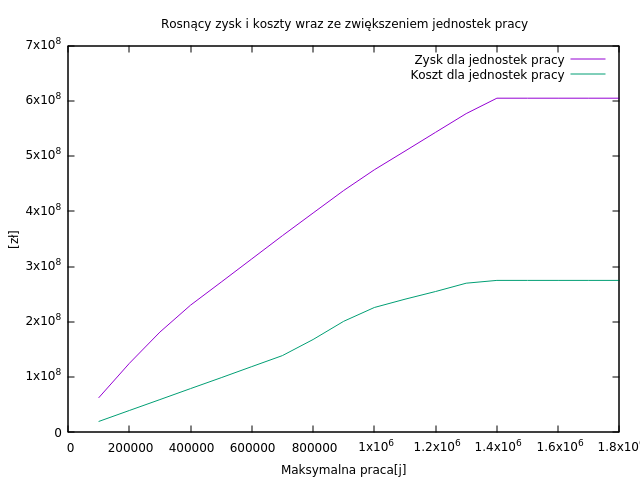
\includegraphics[width=0.99\textwidth]{output/chart.png} % scales both width and height by 0.5
\end{figure}

Wnioski:

\begin{itemize}
    \item Zasoby pracy były zawsze wykorzystywane aż do limitu 1.4e+06, w którym to zostało zużyte 1.39e+06 jednostek pracy. 
    \item W większości przypadków maksymalizacja zysku odbywa się poprzez sprzedaż i produkcję ciągników. Jedynym odstępstwem jest przedział $1.3e+06 < $ Maksymalna praca $ < 1.3e+06$ gdzie sprzedawana była również stal. 
      Myślę, że jest to spowodowane brakiem sprzedaży ciągników, które to zaczynają być znowu sprzedawana gdy pojawiają się nowe jednostki pracy. Możliwe, że powodują to wysokie wymagania jednostek pracy oraz jednostek stali do produkcji maszyn. 
    \item W żadnym przypadku możliwości produkcyjne towarów nie zostały przekroczone.
    \item Przy zwiększaniu maksymalnego zasobu pracy powyżej 1.4e+06 można zauważyć, że ciągniki nie są produkowane oraz sprzedawane. Jest to spowodowane ogarniczeniem produkcji maszyn, które osiąga tam 50 tys jednostek.
    \item Po zwiększeniu zasobu pracy do $1.4e+06$ udało się osiągnąć maksymalne możliwości produkcyjne zakładu.
    \item Dodanie wymagania pelnego wykorzystania zasobów pracy nie wpłynęłoby na wyniki ponieważ zasoby pracy zawsze były w pełni wykorzystywane.
    \item Wraz ze wzrostem zasobów pracy rośnie zysk oraz koszt co obrazuje wykres \ref{fig:chart}
\end{itemize}

\section{Analiza  możliwości  rozszerzania  modelu.  Opis  projektu  koncentruje  się  na  opisie uproszczonej  sytuacji  decyzyjnej.  Przedyskutować  możliwości  rozszerzenia  modelu urealniające  jego  zastosowanie  wskutek  uwzględnienia  większej  liczby  zależności  itp. Przeanalizować ewentualne skutki takich rozszerzeń dla zadania obliczeniowego}

Uproszczony model z zadania można rozszerzyć o następujące zależności:

\begin{itemize}
  \item Opisywany model zawiera małą ilość zmiennych. Rozszerzając go do lepszego opisania rzeczywistości możnaby uwzględnić również zmienne opisujące \textbf{zużycie prądu, wody, większe składowe towarów oraz np. powierzchni potrzebnej na wyprodukowanie poszczególnych towarów}. 
    Oprócz takich podstawowych zmiennych można również dodać bardziej skomplikowane jak np. \textbf{uwzględnienie pracy zmianowej, czasu pracy, zmiany cen w czasie czy choćby czas oraz koszt transportu towarów na sprzedaż}. O ile te pierwsze rozszerzenia możnaby łatwo dodać
    do modelu to bardziej skomplikowane wymagałyby znajomości większej ilości algorytmów optymalizacji. Największym problemem do zamodelowania byłaby zmienna związana z czasem. Na pewno jednak sprawiłaby ona, że model byłby zdecydowanie bardziej realistyczny. Wydaje mi się, że
    odpowiednie określenie czasu wymaganego do stworzenia maszyn oraz ciągników mogłoby sprawić, że sprzedaż towarów mogłaby być bardziej różnorodna.
  \item Obecnie model głównie skupia się na sprzedaży jednego produktu co zazwyczaj nie występuje w przedsiębiorstwach. Można by go rozszerzyć dodając ograniczenia powodujące, że wymagane jest sprzedanie określonych ilości towarów a nie tylko limitowanie ich sprzedaży. 
    Z pewnością takie rozwinięcie modelu wpłynęłoby na lepsze opisanie przez niego rzeczywistości i nie powinno znacznie go skomplikować.
  \item Zróżnicowanie sprzedaży można by również zapewnić poprzez rabaty na zakup większej ilości sprzętu podczas jednej tranzakcji sprzedaży oraz wprowadzenie systemu klientów. Zbiór klientów mógłby posiadać ograniczenia ile jednostek surowców można sprzedać.
  \item Aby urealnić model trzeba ograniczyć system jednostek towarów wyprodukowanych do liczb naturalnych. Obecnie model zakłada podzielność jednostek co nie ma pokrycia w rzeczywistości. Odnoszę jednak wrażenie, że nie miałoby to zbyt dużego wpływu na wyniki ponieważ
    bez zróżnicowania sprzedaży za pomocą ograniczeń system nadal maksymalizowałby sprzedaż ciągników.
\end{itemize}




\end{document}
